\documentclass[acmtocl,acmnow]{acmtrans2m}
\usepackage{amssymb}
\usepackage{amsmath}
\usepackage{url}
\usepackage{wrapfig}
\usepackage[usenames]{color}
\usepackage[dvips]{epsfig,psfrag}

%graphics
\newcommand{\ellipse}[1]{{\raisebox{-1ex}{\protect\psfrag{a}[][]{\small$#1$}%
\protect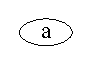
\includegraphics[width=10mm,height=5mm,clip]{vertex.eps}}}}
\newcommand{\Sourcevertex}{{\raisebox{-.2ex}{
\includegraphics[width=3.5mm,clip]{sourcevertex.eps}}}}
\newcommand{\Sinkvertex}{{\raisebox{-.2ex}{
\includegraphics[width=3.5mm,clip]{sinkvertex.eps}}}}
\newcommand{\sourcevertex}{{\raisebox{-.2ex}{
\includegraphics[width=2.5mm,clip]{sourcevertex.eps}}}}
\newcommand{\sinkvertex}{{\raisebox{-.2ex}{
\includegraphics[width=2.5mm,clip]{sinkvertex.eps}}}}

%names and CS terms
\newcommand{\entry}{entry}
\newcommand{\exit}{exit}
\newcommand{\Loop}{loop}
\newcommand{\branch}{branch}
\newcommand{\basicblock}{basicblock}
\newcommand{\OpenAD}{OpenAD}
\newcommand{\OpenADFortTk}{OpenADFortTk}
\newcommand{\OpenAnalysis}{OpenAnalysis}
\newcommand{\OpenSixtyFour}{Open64}
\newcommand{\XAIF}{XAIF}
\newcommand{\xaifBooster}{xaifBooster}
\newcommand{\whirlToxaif}{whirl2xaif}
\newcommand{\xaifTowhirl}{xaif2whirl}

%math
\newcommand{\R}{I\!\!R}
\newcommand{\bmC}{\mbox{\bf\em C}}
\newcommand{\bmf}{\mbox{\bf\em f}}
\newcommand{\bmg}{\mbox{\bf\em g}}
\newcommand{\bmI}{\mbox{\bf\em I}}
\newcommand{\bmJ}{\mbox{\bf\em J}}
\newcommand{\bmu}{\mbox{\bf\em u}}
\newcommand{\bmv}{\mbox{\bf\em v}}
\newcommand{\bmw}{\mbox{\bf\em w}}
\newcommand{\bmx}{\mbox{\bf\em x}}
\newcommand{\bmy}{\mbox{\bf\em y}}

%environments
\newcommand{\reffig}[1]{Figure~\ref{#1}}
\newcommand{\refsec}[1]{Section~\ref{#1}}
\newcommand{\refeqn}[1]{(\ref{#1})}
\newcommand{\refcan}[1]{(C\ref{#1})}
\newtheorem{Can}{Canonicalization}

\markboth{Lots Of Authors et al.}{\OpenAD}

\title{\OpenAD: A tool for automatic differentiation 
of Fortran90 codes}

\author{PATRICK HEIMBACH, CHRIS HILL, DERYA OZYURT, CARL WUNSCH\\Massachusetts Institute of Technology\\
MIKE FAGAN, NATHAN TALLENT \\Rice University\\
MICHELLE STROUT, JEAN UTKE \\Argonne National Laboratory 
\and
UWE NAUMANN\\Rheinisch Westf\"alische Techinische Hochschule Aachen\\
{\color{Red}[ fix the ordering ]}
}

\begin{abstract}
The \OpenAD\ tool allows the evaluation of first and second order 
derivatives of functions defined by a program written in Fortran90/77. 
The derivative evaluation is performed by Fortran 90 code resulting from the 
analyses and transformation of the original program that defines the function of interest.
The code transformation follows the basic principles of automatic differentiation. 
In difference to most other automatic differentiation tools \OpenAD\ is 
built from components that permit an easy extension of the code transformations 
in a language indepdendent fashion. It uses code analysis results implemented 
in the \OpenAnalysis\ component. 
The interface to the language independent transformation 
engine is an xml abstract interface format, called \XAIF\ that is  specified through an xml schema. 
The implemented transformation algorithms allow efficient derivative computations utilizing 
locally optimized cross country  sequences of vertex, edge and face elimination steps. 
Specifically for the generation of adjoint codes \OpenAD\ supports various code reversal 
schemes with hierachical checkpointing at the subroutine level. 
The Fortran specifive front and back end to this transformation engine is the \OpenSixtyFour\ based
\OpenAD\ Fortran tool kit, \OpenADFortTk.
\end{abstract}


\category{G.1.4}{Quadrature and Numerical Differentiation}{Automatic differentiation}
\category{D.3.4}{Processors}{Code generation, Compilers}
\category{F.3.2}{Semantics of Programming Languages}{Program analysis}
\category{G.1.6}{Optimization}{Gradient methods}

\terms{Algorithms, Performance}

\keywords{Automatic differentiation,  source transformation, adjoint compiler}

\begin{document}


\begin{bottomstuff} 
P.~Heimbach, C.~Hill, D.~Ozyurt, and C.~Wunsch, Massachusetts Institute of Technology, 
Boston, MA 02139;\newline
M.~Fagan, N.~Tallent, Rice University, 
Houston, TX 77251;\newline
M.~Strout, J.~Utke, Argonne National Laboratory, 
Argonne, IL 60439;\newline
U.~Naumann, Rheinisch Westf\"alische Techinische Hochschule Aachen, 
D-52056 Aachen, Germany;\newline
Funding for the ACTS project is provided by NSF under ITR contract OCE-0205590
for a three year period that started in September 2002.
\end{bottomstuff}
\maketitle

%#########################################################################################
\section{Introduction} \label{sec:Introduction}

The basic principles of automatic differentiation (AD), see also \refsec{ssec:ADIntro}, 
have been known for several decades \cite{wengert}
but only during the last 15 years the tools implementing AD have found a noticable use in 
optimization, data assimilation, and other applications in need of efficient and accurate 
derivative information. 
As a consequence of the wider use of AD 
a variety of tools have been developed that address specific 
application requirements or programming languages. 
The website {\tt www.autodiff.org} provides a good overview of the tools that 
are currently available. 
One may characterize two user groups of AD tools. On one side are the casual users 
with small scale problems applying AD mostly in a black box fashion and demanding 
minimal user intervention. 
On the other side are experienced AD users aiming for highly efficient 
derivative computations. Their need for efficiency is dictated by the 
computational complexity of models that easily reaches the limits of  current 
supercomputers. With the emphasis on efficiency some sacrifices on the support of 
language features are acceptable for this user group. 

One of the most demanding applications of AD is the computation of gradients for 
data assimilation on large scale models used in oceanography and climate research. 
An evaluation of the available tools revealed some shortcomings from the perspectives 
of the tool users as well as the tool developers. 

From  the AD tool  users point of view ... 
{\color{Red} [ FILL IN ] } 

From the AD tool developers point of view ...
{\color{Red} [ FILL IN ] } 

These issues became the motivation for the 
Adjoint Compiler Technology \& Standards (ACTS) project\footnote{ 
see {\tt www.stce.rwth-aachen.de/ACTS}
}. 
This project is a collaborative
research and development effort between MIT, Argonne National Laboratory, 
Univeristy of Chicago, and Rice University. 
It focusses on  next-generation tool development and 
application of AD to problems in oceanography and chemical engineering.
The main result of this effort is an infrastructure for the language independent 
development and use of AD algorithms. 
\OpenAD\ is the Fotran90 incarnation of the infrastructure.\footnote{
The C/C++ oriented ADIC version 2.0 is based on the same infrastructure and can be found
at {\tt www.mcs.anl.gov/adicserver}.
}
\begin{wrapfigure}{r}{6cm}
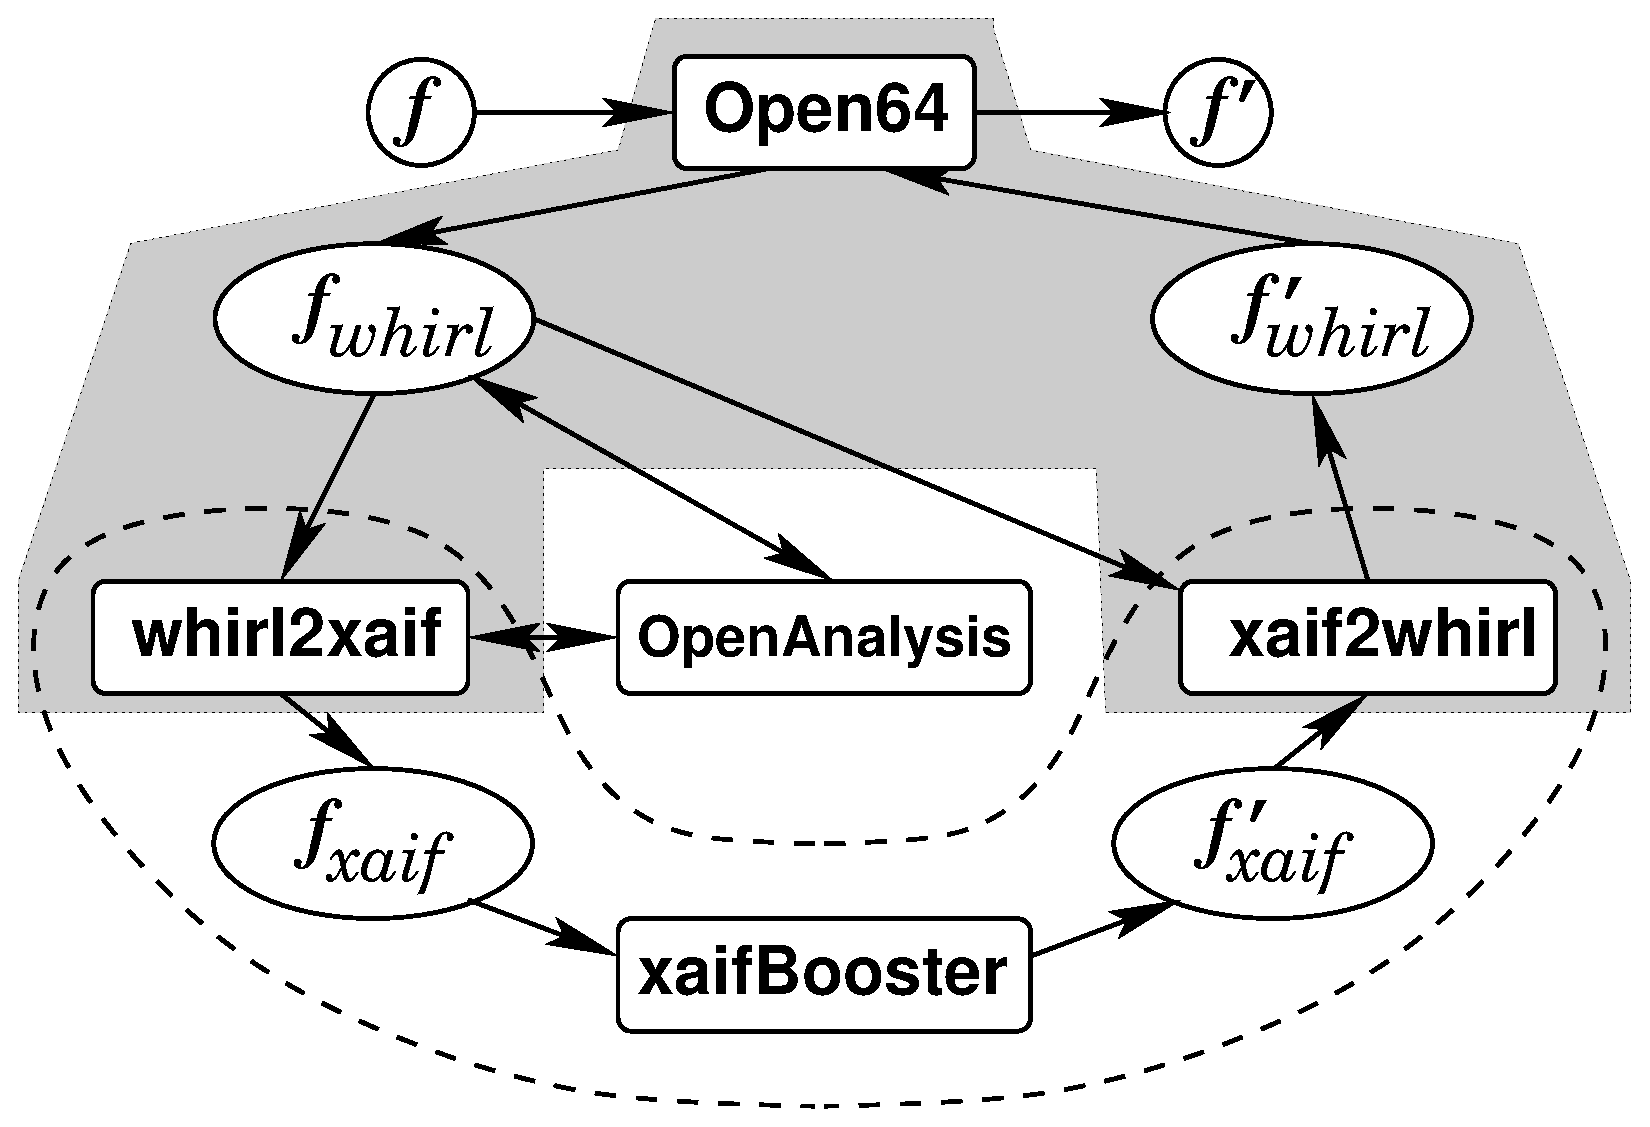
\epsfig{file=overview.eps,width=6cm}
\caption{\OpenAD\ components and pipeline} \label{fig:overview}
\end{wrapfigure}
The collaboration  of the \OpenAD\  components is illustrated in 
\reffig{fig:overview}
The \OpenSixtyFour\ front-end performs a lexical, 
syntactic, and semantic analysis and produces an 
intermediate representation of $F$ in the so-called {\em whirl} format.
\OpenAnalysis\ is used to build call and control flow graphs and  perform 
code analyses such as alias, activity, side-effect analysis.
This information is used by 
\whirlToxaif\ to construct a representation of the numerical core of $F$ in
\XAIF\ format shown as $F_{xaif}$.  
A differentiated version of $F_{xaif}$ is derived by an 
algorithm that is implented in \xaifBooster\ and is again respresented 
\XAIF\ as $F'_{xaif}$.
The information in $F'_{xaif}$ and the original $F_{whirl}$ are used by 
\xaifTowhirl\ to construct a 
{\em whirl} representation $F'_{whirl}$ of the differentiated code. 
The unparser of 
\OpenSixtyFour\ transforms $F'_{whirl}$ into Fortran90, thus completing
the semantic transformation of a program $F$ into
a differentiated program $F'$.
The dotted line encloses the language specific front-end that can potentially
be replaced by front-ends for languages other than Fortran. 
For example, an 
effort running parallel to the ACTS project at Argonne National Laboratory is 
developing a new version of ADIC \cite{HoNo01} by coupling a C/C++ 
front-end 
based on an EDG parser ({\tt www.edg.com}) and uses ROSE in combination with SAGE~3 ({\tt www.llnl.gov/CASC}) as internal representation
with \OpenAD.

This paper discusses the components of \OpenAD,
including the underlying design decisions, algorithmic aspects, and
numerical results.
 
%#########################################################################################
\section{AD Concepts}\label{sec:ADIntro}

In this section we introduce the terminology we will refer to throughout 
this paper. We will also introduce a number of canonicalizations 
that are required to simplify the theoretical and practical 
aspects of the code transformation in \OpenAD.

A detailled introduction to AD can be found in \cite{Gri00}. 
We would also like to refer the reader to the proceedings of four conferences 
on AD \cite{CG91,BBCG96,CFG+01,BCH+05}.

We assume a vector valued function $\bmy=\bmf(\bmx): \R^n\mapsto \R^m$ that is implemented 
as a computer program in a language such as Fortran, C, or C++. 
The computer program 
induces a {\em call graph} (CG) \cite{Aho}
whose vertices are subroutines and whose edges 
represent calls potentially made during the computation of $\bmy$ for particular 
values of $\bmx$. 
Every subroutine consists of a {\em control flow graph} (CFG) that 
represents the typical control flow constructs such as \entry, \exit, \Loop, \branch, 
and \basicblock. 
A \basicblock\ consists of a sequence of assignments and subroutine calls. 
In the following we assume some canonicalizations are performed. 
These canonicalizations are implemented in the front end discussed in 
\refsec{sssec:Canonicalization}.
\begin{Can} \label{can:funcToSub}
All constructs occuring in \basicblock\ that are neither assignments nor subroutine calls (such as function calls, built-in I/O statements) 
are canonicalized into subroutine calls.
\end{Can}
\begin{Can} \label{can:assignSideEffectFree}
An assignment effects a single variable on the left-hand side and 
the right-hand-side expression is side-effect free.
\end{Can}
\begin{Can} \label{can:assignElemental}
The right-hand-side expression consists only of elemental operations $\phi$ typically 
defined in a programming language as built-in operators and intrinsics.
\end{Can}
\begin{Can} \label{can:assignFunction}
User defined functions and calls to these functions in right-hand-side expressions 
are canonicalized to subroutined calls.
\end{Can}
Without loss of generality we can assume that an evaluation of $\bmf(\bmx)$ for  
a particular value of $\bmx$ can be represented by a sequence of 
elemental operations $v_j=\phi_j(\ldots,v_i,\ldots)$. 
The $v_i$ represent the vertices $\in V$ in the correspong corresponding computational 
graph $G=(V,E)$. The edges $(i,j)\in E$ in this graph are the direct dependencies 
implied by the elemental $v_j=\phi_j(\ldots,v_i,\ldots)$.

The elemental operations $\phi$ are differentiable on open subdomains. 
Each edge $(i,j)\in E$ has an attached local partial derivative 
$c_{ji}=\frac{\partial v_j}{\partial v_i}$. 
The central principle of AD is 
the application of the chain rule to the elemental $\phi$, that is 
multiplications and additions of the  $c_{ji}$.  

Because the code for a $\bmf$ generally contains control flow constructs there is no 
single $G$ that represents the computation of $\bmf$ for all possible values of $\bmx$.

In practice, \OpenAD\ considers subgraphs constructed 
from the contents of a \basicblock.
In the following we illustrate the prinicpal approach with the use 
of a toy example.  
\begin{wrapfigure}{l}{.5\linewidth}
\begin{tabbing}
\hspace{.6cm}{\footnotesize \bf 01}\hspace{.5cm} {\tt y(k)=sin(x(1)*x(2)); k=k+1} \\
\hspace{.6cm}{\footnotesize \bf 02}\hspace{.5cm} {\tt if} \={\tt (mod(k,2) .eq. 1) then } \\
\hspace{.6cm}{\footnotesize \bf 03}\hspace{.5cm} \>{\tt y(k)=2*y(k-1)}  \\
\hspace{.6cm}{\footnotesize \bf 04}\hspace{.5cm} {\tt else } \\
\hspace{.6cm}{\footnotesize \bf 05}\hspace{.5cm} \>{\tt do} \={\tt i=1,k } \\
\hspace{.6cm}{\footnotesize \bf 06}\hspace{.5cm} \>\>{\tt t1=x(1)+x(2) } \\
\hspace{.6cm}{\footnotesize \bf 07}\hspace{.5cm} \>\>{\tt t2=t1*sin(x(1)) } \\
\hspace{.6cm}{\footnotesize \bf 08}\hspace{.5cm} \>\>{\tt x(1)=cos(t1*t2) } \\
\hspace{.6cm}{\footnotesize \bf 09}\hspace{.5cm} \>\>{\tt x(2)=-sqrt(t2) } \\
\hspace{.6cm}{\footnotesize \bf 10}\hspace{.5cm} \>{\tt end do } \\
\hspace{.6cm}{\footnotesize \bf 11}\hspace{.5cm} {\tt end if } \\
\hspace{.6cm}{\footnotesize \bf 12}\hspace{.5cm} {\tt y(k)=y(k)+x(1)*x(2) } 
\end{tabbing}
\caption{Toy example code}\label{fig:toy}
\end{wrapfigure}
Line numbers have been added for simpler referencing within the text.
The CFG resulting from the above code is depicted in 
\reffig{fig:cfg}(a).
The assignment statements are contained in the {\basicblock}s B(2,3,4,6,12).
For instance, 
the statements  in the lines 06--09 form the loop body, \basicblock\ B(6).
As B(6) is executed
{\tt k} times it may be worth putting
additional effort into the optimization of the derivative code 
generated for B(6).
\begin{figure}[ht]
\centering
\begin{tabular}{ccc}
\epsfig{file=cfg_ts.ps,width=.303\textwidth} &
\epsfig{file=cfg_tape.ps,width=.303\textwidth} &
\epsfig{file=cfg_adj.ps,width=.31\textwidth} \\
\em (a) & \em (b) & \em (c)
\end{tabular}
\caption{CFG of \reffig{fig:toy} (a) original code, (b) tangent linear model, (c) adjoint model}\label{fig:cfg}
\end{figure}
For B(6) the corresponding computational graph $G$  is depicted in 


Conceptually, AD is based on a decomposition of the evaluation routine for
$\bmf$ into a three-address code\footnote{We assume that there are at most binary
arithmetic operators and intrinsic functions. The generalization is trivial.}
of the form
\begin{equation} \label{eqn:tac}
v_j = \varphi_j(v_i,v_h)
\end{equation}
for $j=1,\ldots,q$ and $h,i=1-n,\ldots,q,$ $j>h,i.$ The $n$ {\em independent}
variables $x_1,\ldots,x_n$ correspond to $v_{1-n},\ldots,v_0.$ We consider the 
computation of the first derivative of the {\em dependent} variables 
$y_1,\ldots,y_m$ represented by $m$ variables $v_j: j \in 1-n,\ldots,q$
with respect to the independents. The resulting $m \times n$ matrix is known
as the {\em Jacobian matrix} of $\bmf.$

The {\em elemental} functions $\varphi_j,$ $j=1,\ldots,q,$ are assumed to have 
jointly continuous partial derivatives in a neighborhood of the current 
argument. The values of these partials can be computed in parallel with the 
function itself for given values of the independent variables.
Consequently, the {\em forward mode} of AD propagates directional derivatives
as 
\begin{equation} \label{eqn:fm}
\dot{v}_j= \frac{\partial \varphi_j}{\partial v_h}(v_i,v_h) * \dot{v}_h + \frac{\partial \varphi_j}{\partial v_i}(v_i,v_h) * \dot{v}_i \quad \text{for}~~j=1,\ldots,q.
\end{equation} 
In {\em reverse mode} we compute adjoints of the variables on the right-hand 
side in \refeqn{eqn:tac} as a function of local partial derivatives and the 
adjoint of the variable on the left-hand side:
\begin{equation} \label{eqn:rm}
\begin{split} 
\bar{v}_i&=\bar{v}_j * \frac{\partial \varphi_j}{\partial v_i}(v_i,v_h) \\
\bar{v}_h&=\bar{v}_j * \frac{\partial \varphi_j}{\partial v_h}(v_i,v_h) \\
\end{split} 
\quad 
\text{for}~~j=q,\ldots,1-n.
\end{equation} 

Equations (\ref{eqn:fm}) and (\ref{eqn:rm}) can be used to accumulate the Jacobian of $\bmf$ at a computational complexity that is proportional to
$n$ and $m,$ respectively. One simply lets $\dot{\bmx}$ or $\bar{\bmy}$ range
over the Cartesian basis vectors in $\R^n$ or $\R^m.$
Basic blocks can be considered as vector functions themselves. 
Forward and reverse mode AD,
or, as we will see below, local combinations of the two, can be applied to
compute the local Jacobians. If $\bmy=\bmf(\bmx)$ is computed by
a sequence of basic blocks $F_1,\ldots,F_l$ and assuming the availability
of the local Jacobians 
$F'_1,\ldots,F'_l,$ then 
equations~(\ref{eqn:fm}) and (\ref{eqn:rm}) can be generalized as follows:
\begin{equation} \label{eqn:bbfm}
\dot{y}_j=F'_j \dot{x}_j \quad \text{for}~~j=1,\ldots,l
\end{equation} 
and 
\begin{equation} \label{eqn:bbrm}
\bar{x}_j=(F'_j)^T \bar{y}_j \quad \text{for}~~j=l,\ldots,1\quad ,
\end{equation} 
where $x_j = (x^j_i \in V :  i=1,\ldots,n_j)$ and
$y_j = (y^j_i \in V : i=1,\ldots,m_j)$ are the inputs and outputs of $F_j,$
respectively. 

The control-flow graph of the example is shown in \reffig{fig:cfg}~(a).
Assuming that code for accumulating the local Jacobians $F'_1, \ldots, F'_4$
of the basic blocks $F_1,\ldots,F_4$ is available (some aspects of how to generate
such code automatically and how to optimize it is the subject of this paper), 
the  forward and reverse modes of AD compute products
of the Jacobian and its transposed with a vector, respectively. In 
\reffig{fig:cfg}~(b) products of the local Jacobians $F'_i$ 
with the directions $\dot{x}_i$ in the input space of each basic block 
$F_i,$ $i=1,\ldots,4,$
are propagated forward in the direction of the flow of control. 
The direction is reversed in reverse mode. Products of the transposed
Jacobians $(F'_i)^T$ with adjoint vectors in the respective output spaces
are propagated reverse to the direction of the flow of control. In \reffig{fig:cfg}~(c) we have
switched the orientation of the edges to illustrate this fact.

To finish this introductory example, we make the following 
important point: Thanks to the associativity of the chain rule it is
possible to {\em preaccumulate} derivative information of certain parts
of the code and use this information in the propagation of directional
derivatives (in forward mode) or adjoints (in reverse mode). Occasionally
it is worthwhile to put additional effort into the optimization of this
preaccumulation code. In this paper we discuss various issues arising from
the optimization of Jacobian code in the context of automatic source 
transformation techniques.
%%%%%%%%%%%%%%%%%%%%%%%%%%%%%%%%%%%%%%%%%%%%%%%%%%%%%%%%%%%%%%%%%%%%%%%%%%%%%%
\subsection{Elimination Methods} \label{ssec:tools}
Let $\bmf$ represent a basis block that is subject to preaccumulation
as outlined in the previous section.
The DAG  $G=(V,E)$ is induced by the code for $\bmf$ \cite{ASU86}.
We use a numbering scheme with $n$ independent vertices 
$x_1=v_{1-n},\ldots,x_n=v_0 \in X$, 
$p$ intermediate vertices 
$v_1,\ldots,v_p \in Z$,  
$m$ dependent vertices 
$y_1=v_{p+1},\ldots,y_m=v_{p+m} \in Y$, 
representing the corresponding independent, intermediate, and dependent 
variables.
For notational simplicity and without loss of generality we assume that the 
dependent variables are mutually independent. This situation can always be
reached by introducing auxiliary assignments.
Consequently, $V=X\cup Z \cup Y$. 
The numbering is subject to the dependence relation 
$\prec$, where $v_i \prec v_j$ (and 
$v_h \prec v_j$ as in \refeqn{eqn:tac}), and
$ v_i \prec v_j \Rightarrow i<j.$
\begin{figure}[ht]
\centering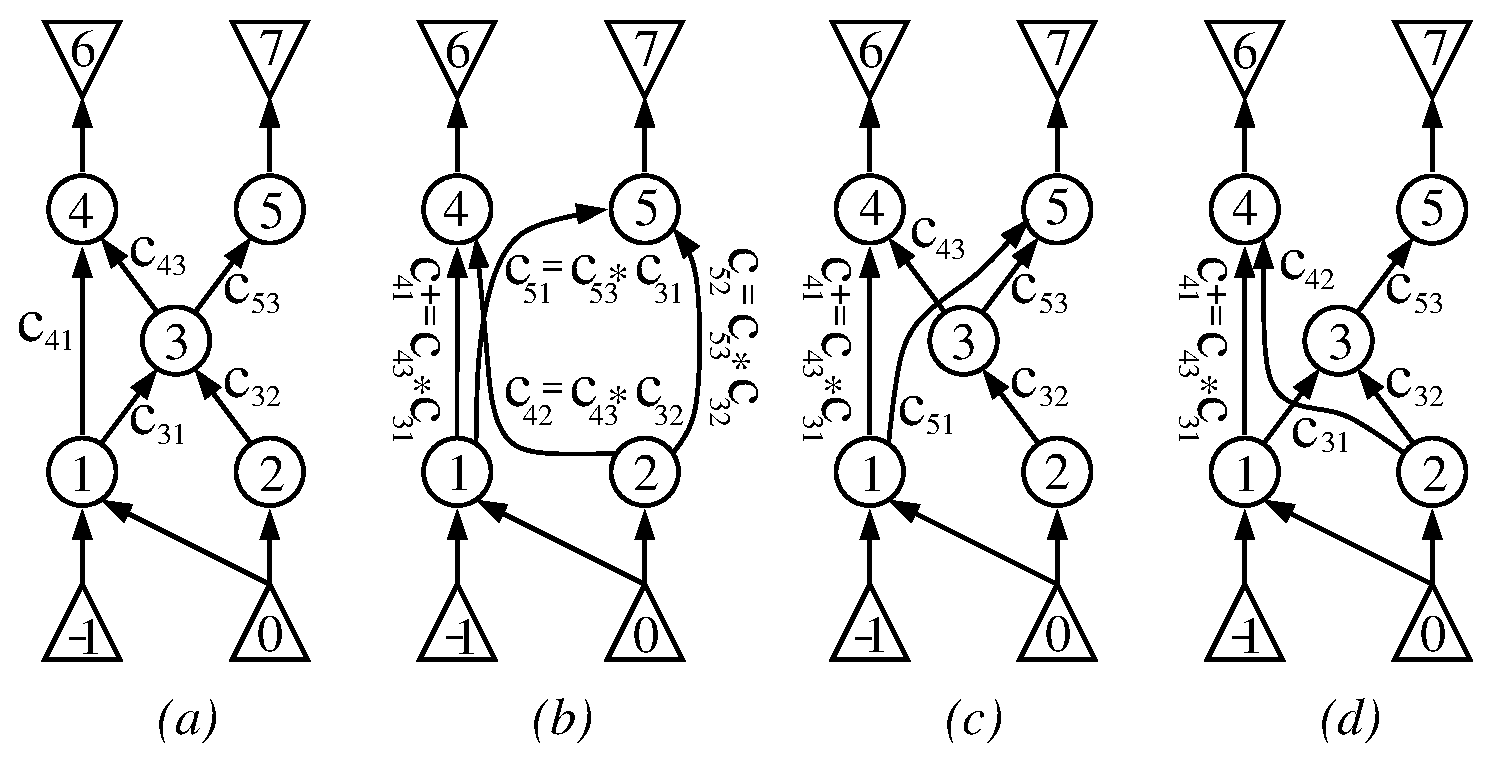
\epsfig{file=elims.eps,width=.7\linewidth}
\caption{
(a) Computational graph $G$ for \refeqn{eqn:sampleCode}, 
(b) vertex elimination $G-3$, 
(c) edge-front elimination $G-(1,3)$, 
(d) edge-back elimination $G-(3,4)$} 
\label{fig:elims}
\end{figure}
In \reffig{fig:elims}~(a) we show the DAG for $F_3$ from the previous section. 
It represents a decomposition of the code into a sequence assignments of
the results of the elemental operations $\varphi$ to unique intermediate 
variables,
for example,
\begin{equation}\label{eqn:sampleCode}
\begin{split}
 v_1&=v_{-1}+v_0;~v_2=\sin(v_0);~v_3=v_1+v_2;~v_4=v_1*v_3; \\
v_5&=\sqrt{v_3};~v_6=\cos(v_4);~v_7=-v_5 \quad .\\
\end{split}
\end{equation}
This representation is also referred to as the {\em code list}.
The intrinsics and operators provided by the underlying programming language 
constitute the possible elemental operations.
Edges $(i,j)\in E$ are labeled with partial derivatives
$c_{ji}=\frac{\partial \varphi_j}{\partial v_i} \in \R$ of the elemental operations
associated with vertex $j$ with respect to the corresponding arguments. 
For instance, in the 
example we have $c_{64}=-\sin(v_4)$.
All edge labels form the matrix
\[ 
\bmC(\bmx):\R^n\mapsto \R^{(p+m)\times(n+p)}\quad .
\]
The computation of the 
Jacobian $\bmf'(\bmx)$
can be interpreted 
as an elimination sequence in $\bmC$:
\[
\sigma: \R^{(p+m)\times(n+p)} \mapsto \R^{m\times n}\quad .
\]
Equivalently, $\sigma$ transforms $G$ into a bipartite graph $\sigma(G)$ whose 
edge labels are the nonzero elements of $\bmf'$. Alternatively,
Gaussian elimination can be applied to the {\em extended Jacobian} 
$\bmC - \bmI,$ where $\bmI$ is the identity as shown, for example, in 
\cite{Gri00}.


The graph-based elimination steps are categorized in vertex, edge, and face 
eliminations. 
In $G$ a vertex $j \in V$ is eliminated by connecting its predecessors with
its successors \cite{GrRe91}.
An edge $(i,k)$ with
$i \prec j$ and $j \prec k$ is labeled with
$c_{ki}+c_{kj} \cdot c_{ji}$ if it existed before the elimination of $j.$
We say that {\em absorption} takes place.
Otherwise, $(i,k)$ is generated as {\em fill-in} and labeled
with $c_{kj} \cdot c_{ji}$
The vertex $j$ is removed from
$G$ together with all incident edges. 
\reffig{fig:elims}~(b) shows the result of eliminating vertex $3$
from the graph in \reffig{fig:elims}~(a).

An edge $(i,j)$ is {\em front eliminated} by connecting $i$ with all successors
of $j$, followed by removing $(i,j)$ \cite{ElimTechAD2000}.
The corresponding structural modifications of the c-graph in
\reffig{fig:elims}~(a) are shown in
\reffig{fig:elims}~(c) for front elimination of $(1,3).$
The new edge labels are given as well.
Edge-front elimination eventually leads to intermediate vertices in $G$
becoming
{\em isolated}; that is, these vertices no longer have predecessors.
Isolated vertices are simply removed from $G$ together
with all incident edges.

Back elimination of an edge
$(i,j) \in E$ results in connecting all predecessors of $i$
with $j$ \cite{ElimTechAD2000}.
The edge $(i,j)$ itself is removed from $G.$
The back elimination of $(3,4)$ from the graph in \reffig{fig:elims}~(a) 
is illustrated in \reffig{fig:elims}~(d). 
Again, vertices can become isolated as a result of edge-back elimination
because they no longer have successors.
Such vertices are removed from $G.$

Numerically the elimination is the application of 
the chain rule, that is, a sequence of {\em fused-multiply-add} (fma) operations
\begin{equation}\label{eqn:fma}
c_{ki}=c_{ji}*c_{kj}\hspace*{1ex}(+c_{ki}) \hspace*{2ex}\leftarrow \mbox{optional}
\end{equation}
where the additions take place in the case of absorption or fill-in is created 
as described above.

Aside from special cases a single vertex or edge elimination will result in more
than one fma. {\em Face elimination} was introduced 
as the elimination operation with the finest granularity of exactly 
one multiplication\footnote{Additions are not necessarily directly coupled.} 
per elimination step.

Vertex and edge elimination steps have an 
interpretation in terms of vertices and edges
of $G$, whereas face elimination is performed on 
the corresponding directed line graph $\cal G$.
Following \cite{ElimTechMP}, we define the directed line graph $\cal G=(V,E)$ 
corresponding to $G=(V,E)$ as follows:
$${\cal V}=
\{\ellipse{i,j} : (i,j)\in E\} \cup 
\{\ellipse{\sourcevertex,j}:v_j \in X\} \cup 
\{\ellipse{i,\sinkvertex}:v_i \in Y\}$$ and 
\begin{align*}
{\cal E}&=\{(\ellipse{i,j},\ellipse{j,k}): (i,j),(j,k) \in E\} \\
&\cup \{(\ellipse{\sourcevertex,j},\ellipse{j,k}): v_j\in X \wedge (j,k)\in E\} \\
&\cup \{(\ellipse{i,j},\ellipse{j,\sinkvertex}): v_j\in Y \wedge (i,j)\in E\} 
\quad . \\
\end{align*}
That is, 
we add a source vertex \Sourcevertex\ and a sink vertex 
\Sinkvertex\ to $G$ connecting all independents to \Sourcevertex\
and all dependents to \Sinkvertex. $\cal G$ has   
a vertex $ v \in \cal V$ for each edge in the extended $G$, 
and $\cal G$ has an edge $ e \in \cal E$ for each 
pair of adjacent edges in $G$. \reffig{fig:face_elims} gives an 
example of constructing the directed line graph in (b) from the graph in (a).   
All intermediate vertices $\ellipse{i,j} \in \cal V$ inherit the labels  
$c_{ji}$. In order to formalize face elimination, it is advantageous to move away
from the double-index notation and use one that is based on a topological
enumeration of the edges in $G.$ Hence, ${\cal G}=({\cal V}, {\cal E})$ 
becomes a DAG with ${\cal V} \subset I\!\!N$ and
${\cal E} \subset I\!\!N \times I\!\!N$ and
certain special properties.
The set of all predecessors of $j \in {\cal V}$ is denoted as $P_j.$ 
Similarly, $S_j$ denotes the set of its successors in $\cal G.$ 
A vertex 
$j \in \cal V$ is called {\em isolated} if either 
$P_j=\emptyset$ or
$S_j=\emptyset.$ 
Face elimination is defined in \cite{ElimTechMP}
between two incident intermediate vertices $i$ and $j$ in $\cal G$ as follows:
\begin{enumerate}
\item If there exists a vertex $k \in \cal V$ such that $P_k = P_i$ and
$S_k = S_j,$ then
set $c_k = c_k + c_j c_i$ {\em (absorption)};
else ${\cal V}={\cal V} \cup \{k'\}$ with a new vertex $k'$ such that
$P_{k'} = P_i$ and $S_{k'} = S_j$
{\em (fill-in)} and labeled with $c_{k'} = c_j c_i.$
\item Remove $(i,j)$ from $\cal E.$
\item Remove $i \in \cal V$ if it is isolated. Otherwise, if there exists a vertex $i' \in \cal V$ such that
$P_{i'} = P_i$ and $S_{i'} = S_i,$ then
\begin{itemize}
\item set $c_i=c_i + c_{i'}$ {\em (merge)};
\item remove $i'.$
\end{itemize}
\item Repeat Step 3 for $j \in \cal V.$
\end{enumerate}
In \reffig{fig:face_elims}~(c) we show the elimination of $(i,j) \in \cal E$,
where $i=\ellipse{1,3}$ and $j=\ellipse{3,4}$.

\begin{figure}
\centering
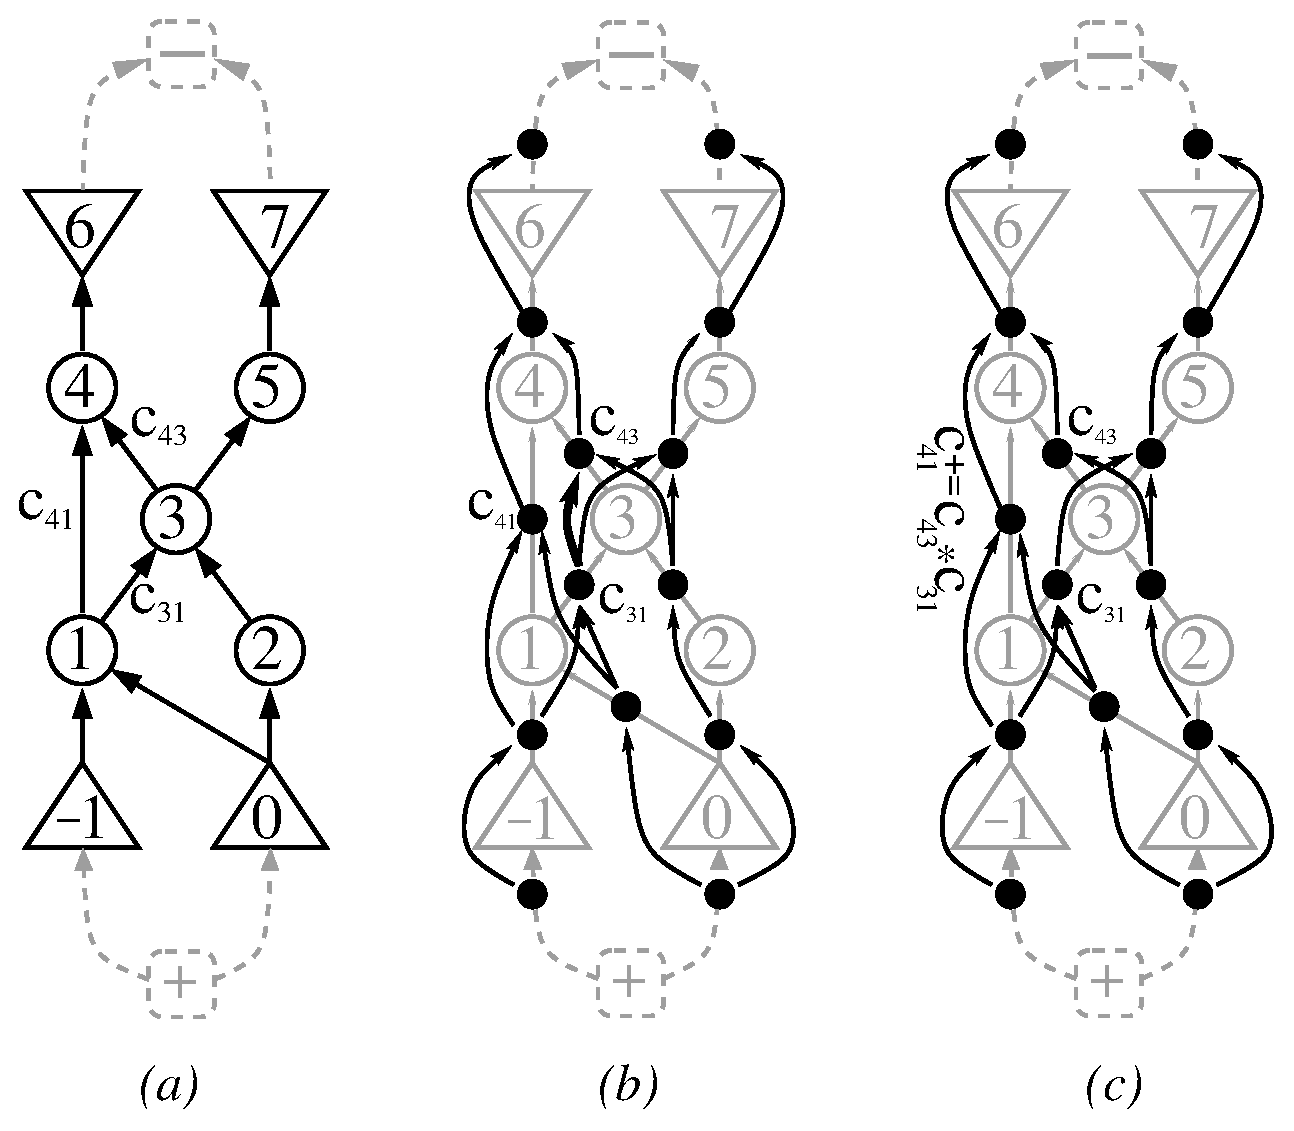
\epsfig{file=face_elims.eps,width=.65\linewidth}
\caption{
(a) $G$ extended, 
(b) $\cal G$ overlaid, 
(c) face elimination 
}
\label{fig:face_elims}
\end{figure}

A complete face elimination sequence $\sigma_f$ yields a tripartite 
directed line graph $\sigma_f({\cal G})$ that can be back transformed into 
the bipartite graph representing the Jacobian $\bmf'$.

In \cite{ElimTechMP} it was shown that vertex and edge 
eliminations can be interpreted 
as groups of face eliminations and that face 
elimination sequences can undercut the number of multiplications of an 
optimal vertex or edge elimination sequence.  
We note that any $G$ can be transformed into the 
corresponding $\cal G$ but that a back transformation 
generally is not  possible once face elimination steps have been applied. 
Therefore, face eliminations cannot precede vertex and edge 
eliminations.

In a source transformation context the operations \refeqn{eqn:fma} are 
expressed as actual code, the Jacobian accumulation code {\tt jac}.
The latter is based on \refeqn{eqn:tac} augmented with statements 
that compute the $c_{ji}$ for all $i \prec j.$
For \refeqn{eqn:sampleCode} we get\footnote{
For better readability we write the indices of the $c_{ji}$ with commas.
} 
\begin{align*}
 v_1&=v_{-1}+v_0;~c_{1,-1}=1;~c_{1,0}=1; \\
 v_2&=\sin(v_0);~c_{2,0}=\cos(v_0); \\
 v_3&=v_1+v_2;~c_{3,1}=1;~c_{3,2}=1; \\
 v_4&=v_1*v_3;~c_{4,1}=v_3;~c_{4,3}=v_1; \\
 v_5&=\sqrt{v_3};~c_{5,3}=(2\sqrt{v_3})^{-1}; \\
 v_6&=\cos(v_4);~c_{6,4}=-\sin(v_4); \\
 v_7&=-v_5;~c_{7,5}=-1; \quad .
\end{align*}
As most of the intermediate variables are used only once, their
creation and assignment should be avoided by the source transformation tool.
However, they are helpful for illustrative purposes as {\tt jac} can
be written in terms of these auxiliary variables.
For example, forward vertex elimination, that is, the elimination
sequence (1,2,3,4,5) in $G$ (\reffig{fig:elims}), leads to the
following Jacobian accumulation code:
\begin{align*}
1:\quad  &c_{3,-1}=c_{3,1} * c_{1,-1};~c_{3,0}=c_{3,1} * c_{1,0};~c_{4,-1}=c_{4,1} * c_{1,-1};~c_{4,0}=c_{4,1} * c_{1,0}; \\
2:\quad  &c_{3,0}\mbox{+=}c_{3,2} * c_{2,0}; \\
3:\quad  &c_{4,-1}\mbox{+=}c_{4,3} * c_{3,-1};~c_{4,0}\mbox{+=}c_{4,3} * c_{3,0};~c_{5,-1}=c_{5,3} * c_{3,-1};~c_{5,0}=c_{5,3} * c_{3,0}; \\
4:\quad  &c_{6,-1}=c_{6,4} * c_{4,-1};~c_{6,0}=c_{6,4} * c_{4,0}; \\
5:\quad  &c_{7,-1}=c_{7,5} * c_{5,-1};~c_{7,0}=c_{7,5} * c_{5,0} \quad .
\end{align*}
\pagebreak
For convenience we use the increment operation $\mbox{+=}$ known from C.
A practical measure for the cost of computing 
$\bmf'=\sigma(\bmC(\bmx))$ is 
the count of multiplications $\#_*$ of edge labels. 
The cost of the forward vertex elimination sequence\footnote{Note
that the cost of computing the Jacobian by the classical forward and reverse 
modes is $n*|E|$ and $m*|E|,$ respectively. For \protect\refeqn{eqn:sampleCode} we have $n=m=2$ and
$|E|=10.$ Forward (resp. reverse) vertex elimination is equivalent to the 
{\em sparse} forward (resp. reverse) mode of AD \protect\cite{Gri00}.}
above is 13.
In \refsec{sec:Observations} we discuss other options for measures.


For the source transformation performed by \OpenAD\ we have to ensure that 
$G$ is valid for all possible values of $\bmx$. 




 








%#########################################################################################
\section{\OpenAD\ components}
%-----------------------------------------------------------------------------------------
\subsection{xaif} 
An XML-based ({\tt www.w3c.org/XML}) hierarchy of directed graphs, referred to as xaif 
\cite{HNN02}, is used for the 
internal representation of the numerical core of the implementation
of a given vector function. This format is 
well suited to represent the results of  semantic transformations including 
preaccumulation \cite{BiHa96,CDB96,GrRe91} and 
program reversal \cite{Gri92,WaGr01} at various levels (call graph, control 
flow graphs, basic blocks, expressions). 
The main idea behind xaif is to provide a language-independent exchange
format that separates language-specific from transformation-related 
algorithmic issues. Potentially, front-ends for various programming languages 
can utilize xaif, for example, \OpenSixtyFour\ and EDG/SAGE~3 as pointed out before.

%-----------------------------------------------------------------------------------------
\subsection{\xaifBooster} 
\begin{figure}
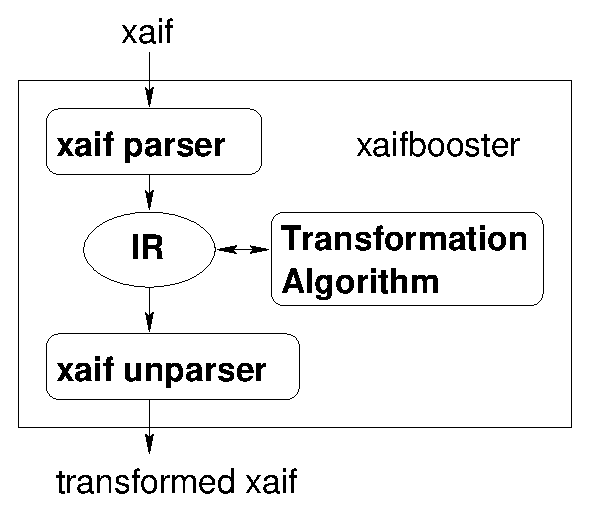
\epsfig{file=principle.eps,width=4cm}
\caption{\xaifBooster\ parses xaif code into an internal representation (IR).
It provides an API for transformation algorithms to modify the IR. An unparser
returns the transformed xaif code.} \label{fig:xaifBooster}
\end{figure}
The C++ code \xaifBooster\ is a collection of utilities and routines for the
(semantic) transformation of programs given in xaif. Its principal architecture 
is illustrated in \reffig{fig:xaifBooster}. One of the major concerns during
the development of \xaifBooster\ has been the clean separation of the internal
representation (an enhanced object image of xaif) from algorithms that operate 
on this data structure. This goal has been achieved by applying the design 
patterns \cite{DesignPatterns} factory, visitor, and decorator as described in \cite{UtNa03}.
The result is an API that gives AD developers the opportunity
to implement new algorithms in a source transformation environment without
having to implement full compiler front- and back-ends. Building on
this API, we have implemented a tangent-linear algorithm that uses statement-
\cite{SEUpreacc} and basic-block-level preaccumulation of local 
gradients/Jacobians. Near-optimal face elimination \cite{ElimTechMP} sequences 
are computed by the software tool 
ANGEL \cite{AGN03,SAGA} ({\tt angellib.sourceforge.net}) and transformed into 
Jacobian code by
an \xaifBooster\ algorithm. A simple adjoint version of the code is obtained
by taping the local Jacobians 
and by computing the corresponding ``transposed Jacobian-vector" products 
during an interpretive reverse sweep through the tape. This approach is
essentially equivalent to split program reversal \cite{Gri00} and allows
for an easy coupling of tangent-linear and adjoint versions of small to 
medium-sized codes as described in \cite{NaHe03}. 

Details of the automatic generation of adjoint code in split mode are presented
in the full version of the paper. Furthermore, additional information is 
provided on \xaifBooster\ as a platform for implementing new AD algorithms with 
the objective to establish an open quasi-standard development infrastructure
within the AD community.
%-----------------------------------------------------------------------------------------
\subsection{OpenADFortTK (a.k.a. Fortran~90 front-end)}

{\tt ADDED BY MIKE AND NATHAN }

The main target application of the ACTS project is the MIT general
circulation model (MITgcm) \cite{mars-eta:97b,mars-eta:97a}.
It is mostly implemented in Fortran~77 to permit maintenance of an
efficient and correct adjoint as the code evolves \cite{HHG02}. Future
development will increasingly add Fortran~90 features.  The
OpenADFortTK --- OpenAD Fortran Toolkit --- component covers the
Fortran 90-specific features of the OpenAD system. Throughout this
paper, we use ``front-end'' as a synonym for OpenADFortTK.

In spite of the appellation ``front end'', OpenADFortTK subcomponents
operate at several stages of the AD process (as seen in the diagram):

   \begin{description}
     \item[mfef90] A classical compiler front end that parses
       Fortran 90, generating an intermediate representation (IR)
       in the Whirl language

     \item[canonicalizer] Convert some tedious (for AD) 
        programming constructs into canonical form. This component
        is whirl to whirl.

     \item[whirl2xaif] A bridge component that:
        \begin{itemize}
           \item Drives the various program analyses (see OpenAnalysis)
        
           \item Filters out program statements that are not in the
                 computational core of the language.

           \item Converts the program analyses and core computational
                 statements from whirl into XAIF
        \end{itemize}

     \item[xaif2whirl] A bridge component that converts the 
        differentiated program represented in XAIF
        to a whirl representation.

     \item[whirl2f] The ``unparser'' that converts whirl to
        Fortran 90

     \item[postprocessor] Final part of the transformation that
        performs template expansion as well as inlining substitutions.

   \end{description}

Both mfef90 and whirl2f are part of the Open64 project.

In the remainder of this section, we will briefly summarize the
subcomponents.

\subsubsection*{Open64 components}
The Open64 project supplies 2 elements for the front end:
   \begin{enumerate}
      \item mfef90
      \item whirl2f
   \end{enumerate}

To ensure robustness of the AD tool, we sought industrial strength
programming-language-dependent components.  We chose the Center for
High Performance Software Research's (Rice University) \OpenSixtyFour\
compiler, a multi-platform version of the SGI Pro64/Open64 compiler
suite, originally based on SGI's commercial MIPSPro compiler ({\tt
hipersoft.cs.rice.edu/OpenSixtyFour/}).  \OpenSixtyFour\'s Fortran~90
front end, mfef90, is a classical compiler parser that reads Fortran
90 source and converts it to an intermediate language called WHIRL.  A
companion tool, whirl2f, unparses WHIRL back to Fortran 90 source
code.  WHIRL, which resembles a typical abstract syntax tree, has been
designed to enable good optimization for high performance computing in
Fortran, C, and C++. See \cite{whirl-stuff} for more details about the
intermediate language. HiPerSoft's main contribution to the Open64
community has been extending the infrastructure to support
source-to-source transformations; thus, it has invested significant
effort in the whirl2f unparser.

The OpenAD project contributed some development of the pragma /
directive mechanism in the Open64 components.

\subsubsection*{Canonicalization}\label{sssec:Canonicalization}
To simplify the development of the AD engine, the front end converts
abd simplifies some programming constructs. In other words, all
program statements that are differentiated are in \emph{canonical}
form. For OpenAD, some of the canonicalizations performed are:

   \begin{enumerate}
      \item Common blocks are converted to modules
      \item user defined functions are converted to subroutines
      \item Non-variable actual parameters are hoisted to
            temporaries
      \item Derived type references are scalarized.
   \end{enumerate}


[ expand on reason for canonicalization ... ]

\subsubsection*{whirl2xaif and xaif2whirl}

The focus of the ACTS project is on translating WHIRL into XAIF
(\whirlToxaif), feeding it to the differentiation engine, and then
back-translating the differentiated XAIF into WHIRL (\xaifTowhirl).
Two distinguishing features of XAIF shape the contours of \whirlToxaif
and \xaifTowhirl.  First, because XAIF represents only the numerical
core of a program, many WHIRL statements and expressions must be
represented using opaque markers and annotations.  
{\tt ***FIXME example*** } 
These opaque objects, which refer to the input WHIRL, are created by
\whirlToxaif and depositied in special XAIF constructs designed for
conveying such information through the differentiation engines.  Given
the original WHIRL and the differentiated XAIF (with the opaque
objects intact), \xaifTowhirl generates new WHIRL representing the
differentiated code. {\tt ***FIXME: build from CFG***}

The second distinguishing characteristic of XAIF is that it represents
programs as common compiler analyses.  For example, a program is a
collection of symbol tables and a call graph where nodes in the call
graph are control flow graphs; control flow graphs contain basic
blocks with statements.  Moreover, symbols, statements and variable
references in XAIF are annotated with information from data flow
analyses suchas alias analysis, define-use chains, and activity
analysis.  \whirlToxaif\ uses the \OpenAnalysis\ analysis package to
collect all of this information before proceeding with the
translation.

See \cite{RiceTechreport}.


\subsubsection*{Postprocessor}
The postprocessor performs various ``cleanup'' operations of the
differentiated code. The 2 most important tasks are:

   \begin{enumerate}
      \item template expansion
      \item inline substitution
   \end{enumerate}

Template expansion is intimately connected with the differentiation
algorithms. Some parts of the code use different recomputation/storage
strategies, as well as different taping patterns. These various
strategies are encoded in Fortran 90 templates, and expanded by the
post processor.

Similarly, some operations introduced by the differentiation process
are coded as function operations. To make these operations work well,
however, they must be substituted inline, replacing the function call.

[ Need examples of templates here (or somewhere) ]

[ Does inlining serve any other purpose besides efficiency?  Yes --
the inlined routines have strange parameter substitution to support
the active data-structures.]

[postprocessor to handle things that are not convenient in WHIRL.]


%-----------------------------------------------------------------------------------------
\subsection{\OpenAnalysis} 

\footnote{No documentation is available yet.  Refer to the
\OpenSixtyFour\ cvs repository under {\tt
hipersoft.cs.rice.edu/Open64} for information on the code.}

The OpenAnalysis toolkit separates program analysis from 
language-specific or back-end specific intermediate representations.
This separation enables a single implementation of domain-specific 
analyses such
as activity analysis, to-be-recorded analysis, and linearity analysis
in both the ADIC and OpenAD Fortran90 tools.  
Currently the OpenAD Fortran toolkit uses standard analyses within 
\OpenAnalysis such as
control-flow graph construction, call graph construction,
alias analysis, reaching definitions, ud- and
du-chains, and side-effect analysis.  Activity analysis has also 
been implemented within \OpenAnalysis.

Activity analysis is performed by \OpenAnalysis based on information
from the Fortran~90 front-end.  The independent and dependent variables of
interest can be communicated to the front-end through the use of pragmas.
The results of the analysis are then 
encoded by the Fortram~90 front-end into XAIF.  The analysis indicates
which variables are active at any time, which memory references are active, 
and which statements are active.

The activity analysis itself is based on the formulation in~\cite{UweTBRPaper}.
The main difference is that the data-flow framework in \OpenAnalysis does not
yet take advantage of the structured data-flow equations.  Activity analysis is
implemented in a context-insensitive interprocedural fashion.


%#########################################################################################
\section{Application}

The reference application for the first prototype of an \OpenAD\ implementation
is a simplified oceanographic box model for investigating
thermohaline circulation. It relates to the
ocean circulation's role in the variability of the climate system,
on time scales of decades to millennia \cite{tzi-ioa:02}.
Previously, the AD tool TAF \cite{GiKa02} 
had been used to generate the derivative
code in both forward and reverse modes.
See \cite{maro-eta:99} for an applications of
TAF's predecessor TAMC to the MITgcm.

\OpenAD\ has been used to generate tangent-linear and 
adjoint versions of the box model. We established numerical identity between
the Jacobians provided by TAF and \OpenAD.
The successful 
application of \OpenAD\ to the box model code is considered as a feasibility 
proof for the overall approach taken by the ACTS project.  
%-----------------------------------------------------------------------------------------
\subsection{Shallow Water Model}
%-----------------------------------------------------------------------------------------
\subsection{Derya's application}
%#########################################################################################
\section*{Conclusion and Future Work}

\OpenAD\ is an AD tool development infrastructure. Its well-separated components
allow developers to focus on various aspects of source-to-source 
transformation AD, including parsing and unparsing of different programming
languages, data and control flow analysis, and (semantic) transformation 
algorithms. The intention of \OpenAD\ is to provide the AD community with 
an open, extensible, and easy-to-use platform for research and development
in the field. Its intention is not to render obsolete existing source transformation
tools such as ADIFOR,\footnote{{\tt http://www.cs.rice.edu/\~\!adifor}} 
the differentiation-enabled NAG Fortran 95 
compiler,\footnote{{\tt http://www.nag.co.uk/nagware/research/ad\_overview.asp}} TAF,\footnote{{\tt http://www.FastOpt.de}} and TAPENADE.\footnote{{\tt http://tapenade.inria.fr:8080/tapenade/index.jsp}} 
Their closer coupling with the language-specific internal representation of 
the program has the potential to make the
exploitation of certain language features easier. \OpenAD\ is supposed to 
complement these tools by providing well-defined APIs to an open internal 
representation that can be used by a large number of AD developers.
Users of AD technology will benefit from the expected wide
variety of combinations of front-ends and algorithms that is made possible
by \OpenAD.

During the remainder of the ACTS project we will focus on the implementation
of robust and efficient data flow algorithms in \OpenAnalysis, including alias, 
define-use and use-define, in-out \cite{Muc97}, 
activity, and to-be-recorded \cite{HNP02} as well as on 
the development of various reverse mode algorithms for parallel MPI codes
combining elements such as preaccumulation and (automatic) checkpointing
\cite{Gri92}. 
A second set of target 
applications in chemical engineering \cite{FTB97} requires combinations of first and 
second derivatives in addition to methods for exploiting structure and sparsity
of the underlying computation. We intend to investigate ways to compute these
combinations efficiently by integrating \OpenAD\ into the relevant 
numerical algorithms.

Ultimately, our aim is to generate correct, efficient, scalable, and easily 
maintainable adjoint code for the MITgcm. The major challenge arises from the
requirement to tackle problems in which derivatives are calculated with respect 
to billions of controls. A combination of the methods outlined above is 
essential to guarantee the successful completion of this highly ambitious
project.

%#########################################################################################
\bibliographystyle{acmtrans}
\bibliography{openad}


\begin{received}
Received May 2005;
\end{received}

\end{document}
